
\subsection{Deformable rising droplets}

In a suspension of deformable particles it is known that the drag force is a function of the shapes of the drops.
To take in account such parameter in averaged models one usually use a force correlation function of the Capillary or Morton number. 
However, such models are valid in very specific scenario and flow condition. 
Another way to take in account the particles' deformation or aspect ratio, would be to solve an equation for the mean particle shapes. 
Then, one can create a drag force closure for various particles' aspect ratio. 

\begin{figure}[h!]
    \centering
    \hfill
    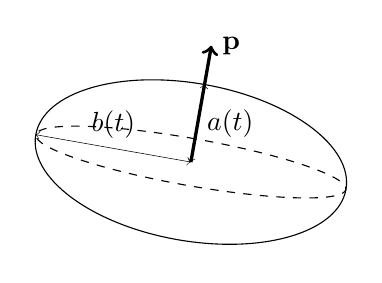
\begin{tikzpicture}[rotate=80]
        \draw(0,0) ellipse (1 cm and 2 cm);
        \draw[dashed](0,0) ellipse (0.3 cm and 2 cm);
        \draw[<->,very thin](0,0) --++ (1,0)node[midway,right]{$a(t)$};
        \draw[->,very thick](0,0) --++ (1.5,0)node[right]{$\textbf{p}$};
        \draw[<->,very thin](0,0) --++ (0,2)node[midway,above]{$b(t)$};
    \end{tikzpicture}
    \hfill
    \caption{Scheme of an  oblate spheroid oriented along the unit vector \textbf{p}.}
    \label{fig:scheme2}
\end{figure}
We consider in this problem an oblate spheroid with a time dependent aspect ratio $\chi = a(t)/b(t)$ oriented along the unit vector \textbf{p}, see \ref{fig:scheme2}.
In this context an equation describing the droplets surface can be found in the reference frame of the droplets, namely, 
\begin{equation}
    \mathscr{F}
    = \textbf{r}\cdot \textbf{H}\cdot \textbf{r} - a_0^2 = 0 
    \label{eq:F_def}
\end{equation}
where \textbf{H} is a symmetric traceless tensor such that $\textbf{H} = \textbf{pp} (a_0/a(t))^2 + (\textbf{I}- \textbf{pp})(a_0/b(t))^2$. 

We consider a mono disperse suspension of droplet with constant mass. 
The objective of this section is to derive constitutive equations to predict the mean orientation, and mean aspect ratio of the droplet. 

\subsubsection{Particle's internal motion}

In the first place we assume a linear homogeneous particle internal motion, such as, 
\begin{equation}
    \textbf{w}_2^0(\textbf{x}_\alpha+ \textbf{r})
    = 
    + \textbf{r} \cdot \textbf{D}_\alpha
    = 
    \bm{\omega}_\alpha \times \textbf{r} 
    + \textbf{r} \cdot \textbf{E}_\alpha
\end{equation}
where $\bm{\omega}_\alpha$ is the angular velocity of the particle, $\textbf{E}_\alpha$ is the mean deformation gradient. 
% Note that the second rank tensor $\textbf{U}_\alpha = \bm{\}$
To respect the mass conservation condition, i.e. $\div \textbf{w}_2^0 =0$, The mean gradient deformation $\textbf{E}_\alpha$ has to respect the conditions : $\textbf{E}_\alpha:\textbf{I}=0$. 
The assumption of linear internal motion is wrong for droplets and bubbles were we are clearly in presence of internal motions. 
However, for now these motions will be discarded. 

\subsubsection{Fundamental properties}

We now compute the mass, moment of mass and moment of momentum of this particle. 
The volume of an ellipsoid reads as, 
\begin{align}
    v_\alpha
    = \frac{4}{3}\pi a b^2
    = \frac{4}{3}\pi \chi  b^3
    \label{eq:volume_def}
\end{align}
Before going further we must say that the two radius $a(t)$ and $b(t)$ are actually dependent since one must preserve the total mass of the particle. 
We recall that we are in the context of mono disperse suspension such that the volume of the particles $v_\alpha$ is actually known, Thus, 
\begin{equation*}
    a(t) 
    = \frac{3 v_\alpha}{4 \pi b^2(t)}
    = \frac{r_0^3}{ b^2(t)}
    \Leftrightarrow
    b^2(t) 
    = \frac{r_0^3}{ a(t)}
\end{equation*}
Where $r_0$ is the radius of the sphere of same volume such as $v_\alpha = \frac{4}{3}\pi r_0^3$. 
Also, it might be useful to compute the relation between the derivative of the radius,  
\begin{equation*}
    \ddt v_\alpha 
    % = \ddt \frac{4}{3}\pi a b^2
    = \frac{4}{3}\pi \dot{a}(t) b^2(t)
    + \frac{8}{3} \pi {a}(t) b(t) \dot{b}(t)
    = 0 
    \Leftrightarrow
     \dot{a}(t)
    =  
    - 2 \frac{a(t)}{b(t)}  \dot{b}(t)
    % \Leftrightarrow
\end{equation*}
Which means that the derivative of both radius are related to twice the aspect ratio. 

The second moment of mass is somewhat more complicated to compute, we have, 
\begin{align*}
    \mathcal{M}_{\alpha,ij}
    = \int r_ir_j dxdydz
\end{align*}
At this stage we would like to compute the integral in spherical coordinate, thus we introduce the change of variables, 
\begin{align*}
    x' = x/a 
    && y' = y/b 
    && z' = z/b 
\end{align*}
By assuming that the spheroid is aligned with the $z$ axis and centered at the origin we get, 
\begin{align*}
    \mathcal{M}_{\alpha,zz}
    = a(t)^3 b(t)^2 \int z'z' dx'dy'dz'
\end{align*}
switching in spherical coordinate yields 
\begin{align*}
    \mathcal{M}_{\alpha,zz}
    = a(t)^3 b(t)^2 \int_0^1 \int_0^{2\pi}\int_0^\pi r^4 \cos^2\phi \sin\phi d\phi d\theta dr
    = a(t)^3 b(t)^2 \frac{1}{5}\frac{4}{3} \pi
    = v_\alpha \frac{a^2(t)}{5}\\
    \mathcal{M}_{\alpha,xx}
    = a(t) b(t)^4 \int_0^1 \int_0^{2\pi}\int_0^\pi r^4 \sin^3\phi\cos^2\theta d\phi d\theta dr
    = a(t) b(t)^4
    \frac{1}{5}
     \frac{4}{3}
     \pi
     =v_\alpha \frac{b^2(t)}{5}
\end{align*}
In a more general manner one can define the tensor $\mathcal{M}_\alpha$ in the laboratory reference frame using the orientation tensor \textbf{p}, such that, 
\begin{equation}
    5 \frac{\mathcal{M}_{\alpha,ij}}{v_\alpha}
    = p_i p_j 
    a^2(t) 
    + (\delta_{ij} - p_ip_j) b^2(t)
    = H_{ij}^{-1}
    \label{eq:M_alpha_def}
\end{equation} 
In light of \ref{eq:M_alpha_def}we reduced the description of any particle in our flow to four parameters, the 3 components of \textbf{p}, and the radius $a(t)$. 
It might be useful to make the inertia tensor dimensionless by dividing both sides by $r_0$, which gives, 
\begin{equation}
    5 \frac{\mathcal{M}_{\alpha,ij}}{v r_0^2}
    = p_i p_j 
    e_{||}^2(t) 
    + (\delta_{ij} - p_ip_j) 
    e_\bot^2(t) 
    \label{eq:M_alpha_def2}
\end{equation} 
Note that since $ab^2 =r_0^3$ the deformation are related through $e_\bot = \frac{b}{a}r e_{||} =\frac{b^3}{r^2} e_{||} $


Now let's compute the first moment of momentum $\mathcal{P}_\alpha$, it reads, 
\begin{align*}
    \mathcal{P}_{\alpha,ij}
    = \int r_i w_{2,j}^0 d\Omega
    = D_{\alpha,jk} \mathcal{M}_{\alpha,ki}
    = \epsilon_{jkl} \omega_{\alpha,k} \mathcal{M}_{\alpha,il}
    +  E_{\alpha,jk} \mathcal{M}_{\alpha,ik}
\end{align*}
Taking the double contracted product with $\epsilon_{mij}$ of the moment of momentum yield the angular momentum equation, 
\begin{align*}
    \mu_{\alpha,m}
    = \epsilon_{mij}\mathcal{P}_{\alpha,ij}
    = \epsilon_{jmi} \epsilon_{jkl} \omega_{\alpha,k} \int r_i r_l  d\Omega
    +  \epsilon_{mij} E_{\alpha,jk} \int r_i r_k  d\Omega\\
    = (\delta_{mk}\mathcal{M}_{\alpha,ll} - \mathcal{M}_{\alpha,mk}) \omega_{\alpha,k}
    +  \epsilon_{mij} E_{\alpha,jk} \int r_i r_k  d\Omega\\
    = \mathcal{I}_{\alpha,mk} \omega_{\alpha,k}
    +  \epsilon_{mij} E_{\alpha,jk} \mathcal{M}_{\alpha,ik}\\
\end{align*}
The second contribution of the angular momentum would vanish if the particles where spherical. 
Lastly, the symmetric part of the moment of momentum reads, 
\begin{align*}
    2\mathcal{S}_{\alpha,ij}
    = \epsilon_{jkl} \omega_{\alpha,k} \mathcal{M}_{\alpha,il}
    + \epsilon_{ikl} \omega_{\alpha,k} \mathcal{M}_{\alpha,jl}
    +  E_{\alpha,jk} \mathcal{M}_{\alpha,ik}
    +  E_{\alpha,ik}  \mathcal{M}_{\alpha,jk}
\end{align*}

\subsubsection*{Evolution equation of a single particle shpae.}

We first start by the kinetic equations.  
In view of the previous expression the evolution equation of the momentum tensor is,  
\begin{equation*}
    \ddt {\mathcal{M}_{\alpha,ij}}
    + \epsilon_{jlk} \omega_{\alpha,k} \mathcal{M}_{\alpha,il}
    - \epsilon_{ikl} \omega_{\alpha,k} \mathcal{M}_{\alpha,jl}
     =  E_{\alpha,jk} \mathcal{M}_{\alpha,ik}
     +  E_{\alpha,ik}  \mathcal{M}_{\alpha,jk}
     \label{eq:dt_M_alpha_bis}
\end{equation*}
On the left-hands-side of \ref{eq:dt_M_alpha_bis} we clearly identify the Jaumann derivative rotating with the vorticity.
To close this equation one may relate the mean ambient flow variables to the particles angular rotation and stretching rate. 
This however this is only possible considering pure stokes flow.

\subsubsection*{Equation for the bulk stress}

The equivalent stress can be formulated as, 
\begin{equation*}
    \bm{\sigma}
    = 
    \phi_1 \bm{\sigma}_1
    + \phi_2 \bm{\sigma}_2
    + \phi_I \bm{\sigma}_I
    \label{eq:sigma_def}
\end{equation*}
The particle phase stress can be reduced to its first moment, $\phi_2 \bm{\sigma}_2 = \pOavg{\bm{\sigma}_2^0}$.
Additionally, we adopt the approximation of homogeneous deformation so that the rate of strain within the particle equal its mean deformation $\textbf{E}_\alpha$.
Thus, we can write 
\begin{equation*}
    \phi_2 \bm{\sigma}_2 
    = - \phi_2 p_2
    + \phi_2 \mu_2 \textbf{E}_p
\end{equation*}
The fluid phase stress can be formulated as $\phi_1 \bm{\sigma}_1 =  - \phi_1 p_1 + \mu_1 \textbf{e} - \mu_1 \phi_2 \textbf{e}_2$.
Likewise, since we considered a constant strain within the particles we can write $\phi_2\textbf{e}_2 = \phi_2 \textbf{E}_p$ in homogeneous medium.   
The previous expression of the averaged stress yields, 
\begin{equation*}
    \bm{\sigma}
    = 
    - p 
    + \mu_1 \textbf{e} 
    + (\mu_2 - \mu_1) \phi_2 \textbf{E}_p
    + \phi_I \bm{\sigma}_I
    \label{eq:sigma_def}
\end{equation*}
In the above stress equation $\bm{\sigma}_I$ is still unknown and must be closed. 
While the others parameters can be easily linked to our problem variable. 

We recall that in homogeneous flows, $\phi_I \bm{\sigma}_I \approx \gamma\pSavg{\textbf{I}-\textbf{nn}}$. 
Let decompose this tensor into an isotropic tensor i.e. $\gamma\pSavg{\textbf{I}-\textbf{nn}} : \textbf{I} \frac{1}{3}I = \gamma\pSavg{} \frac{2}{3} \textbf{I}$ and an anisotropic tensor which reads, $\phi_I \bm{\sigma}_I \approx \gamma\pSavg{\frac{1}{3}\textbf{I}-\textbf{nn}}$.  
Therefore, to close this term one must compute the curvature of the particles. 
The first moment of surface tension stress can be computed analytically following \citep{nadim1996concise} for the curvature computation.
The analytical expression of the ellipse surface will enable us to compute the curvature of each particle.  
Let $\mathscr{F}(\textbf{x},t) = 0$ be the equality representing the ellipsoidal shape of the particle. 
First, the normal pointing in the direction of positive $\mathscr{F}$ at the interface, can be computed as, 
\begin{equation*}
    \textbf{n} = \frac{\grad \mathscr{F}}{(\grad \mathscr{F}\cdot \grad \mathscr{F})^{1/2}} \;\;\text{ on }\;\; \mathscr{F} = 0.  
\end{equation*}
Noticing that $\grad \mathscr{F} = 2\textbf{H}\cdot \textbf{r}$ one obtain, 
\begin{equation*}
    \bm{\sigma}_I^0 =\gamma\left[
    \textbf{I} - \frac{ \textbf{HH} :  \textbf{rr}}{ (\textbf{H}\cdot  \textbf{H}\cdot \textbf{rr})} \right]
\end{equation*}
We recall that this quantity drives the stress jump at the interface. 
As it is expected this stress jump is axis symmetric around the particle main axis. 
Besides, it is maximum at the poles and minimum at the equator of the particle. 
It is then possible to compute the integral of the stress by direct integration in the reference frame of the ellipsoid principal axes. 
The exact result yields, 
\begin{equation*}
    \gamma\pSavg{\textbf{I}-\textbf{nn}}
    = \gamma \left[
        \frac{2}{3} s_\alpha \textbf{I}
        + S (\textbf{I}-\textbf{pp}) -2S\textbf{pp}
        \right]
\end{equation*}
where the first component correspond to the isotropic part of the surface stress, and the second component to the deviatoric part of the surface stress. 
Note that the deviatoric part of this tensor is function of one unique coefficient, $S$ due to the axis symmetrical nature of the droplets. 
Exact solution can be given in terms of the small deformation parameter $e_\bot = b/r$. 
Then an approximation can be deduced for the $e -1 \ll 1$, it gives,
\begin{align*}
    s_\alpha 
    = 4\pi r^2 \left[\frac{e_\bot^2}{2} + \frac{\ln\left(\sqrt{{e_\bot^6}-1}+{e_\bot^3}\right)}{2e_\bot\sqrt{e_\bot^6-1}}\right]
    = 4 \pi r^2 + \frac{24 v }{5 r} (e_\bot-1)^2\\
    S = \frac{4}{3} \pi r^2 \left[
    \frac{\left( \frac{1}{4} - e_\bot^6\right)  \log{\left( \sqrt{e_\bot^6-1}+{e_\bot^3}\right) } }
    { e_\bot  \left( e_\bot^6- 1\right)^{3/2} }
    +  \frac{e_\bot^2\left( e_\bot^6+  \frac{1}{2}\right)}{2\left( e_\bot^6- 1\right)}  \right]
    \approx 
    \frac{8 v}{5 r}(e_\bot-1) + \frac{12 v }{35r}(e_\bot-1)^2 \ldots
\end{align*}
Regarding the expression of the surface of the spheroid, it can be noted that the function within bracket tends to $1$ for $e=1$ leaving us with $s_\alpha = 4\pi r^2$ which is the surface of the sphere. 
Then, it slowly increases when $e$ is either superior or inferior to $1$. 

Equally, the results can be expressed in terms of the deformation parameter $e_{||} = a/r$ in which case the previous results give at the second order in $e_\bot-1$ the following expression, 
\begin{align*}
    s_\alpha 
    \approx 4 \pi r^2 + \frac{6 v }{5 r} (e_{||}-1)^2 \ldots\\
    S 
    \approx 
    - \frac{4 v}{5 r}(e_{||}-1) + \frac{24 v }{35r}(e_{||}-1)^2 \ldots
\end{align*}
Noticing that the Hooke strain tensor $\textbf{C} = (e_{||}-1) \textbf{pp} + (e_\bot-1)(\textbf{I}- \textbf{pp})$, thus one can finally write,
\begin{align*}
    \pSavg{\bm\sigma_I^0}
    = \frac{\gamma v 2}{r} \left[
        1  + \frac{1}{20 }\textbf{C}:\textbf{C}\right] \textbf{I}
        - \frac{\gamma v}{35 r} \left[ 28 \textbf{C}_{-\textbf{I}}
        + 4[\textbf{C}_{-\textbf{I}}\cdot \textbf{C}_{-\textbf{I}} + 15 (\textbf{C}_{-\textbf{I}}:\textbf{pp})^2\textbf{pp}]
        \right]
\end{align*}
This gives the surface stress tensor up to the second order terms in accuracy. 
To our knowledge this has never been proposed. 
Retaining only the first order terms this expression shows that the drop behave as stressed material. 
Indeed, at rest the Laplace pressure is still present. 

It might be interesting to relate teh inertia tensor $\mathcal{M}_\alpha$ and \textbf{C}. 
Indeed, it can be shown that, 
\begin{equation}
    \mathcal{M}_\alpha
     = \frac{v r^2}{5}\left(\textbf{C} + \textbf{I}\right)
\end{equation}
Or equally, 
\begin{equation}
    \textbf{C}
     = \frac{5}{vr^2}\mathcal{M}_\alpha - \textbf{I}
\end{equation}
It is now trivial to re derive \citet{goddard1967nonlinear} equations of motions. 


The only unknown is now the particle strain rate $\textbf{E}_p$ and orientation tensor $\textbf{pp}$ and particle strain tensor \textbf{C} which is only one scalar function. 
\begin{itemize}
    \item Give the Laplace law for elongated bubbles 
    \item \tb{introduce the drop strain from the local strain as it is defined in solid mechanics.}
    \item \tb{TRY TO GET THE SAME EQ as godard}
    \item \tb{DERIVE STRESS EQ WITH C}
    \item The conclusion will be that we could generalize the transport equations or C easli  however we cannot actually close the equaitons for now !! ! 
\end{itemize}

\subsubsection*{Equation for the particles strain}

Additionally, using the first moment of momentum expression one can obtain an other expression for the particles internal stress, 
\begin{equation}
    \intS{ (\bm{\sigma}_I)_{ik}}
    +\intO{ (\bm{\sigma}_2^0)_{ik}}
    = 
    \intO{ \rho_2 
    (\textbf{w}_2^0\textbf{w}_2^0  )_{ik}
    }
    -\ddt \intO{ r_i (\textbf{u}^0_2)_k }
    +\intS{ 
     r_i (\bm{\sigma}_1^0 \cdot \textbf{n}_2)_{k}
    }
\end{equation}

\subsubsection*{Equation for the particle angular momentum}
\begin{equation*}
    \ddt \mu_p = t_p
\end{equation*}